\chapter{Implementation and Test Cases}
\label{ch:impl}
This chapter describes the prototype that implements the methodology of Chapter~\ref{ch:method} and the design of Chapter~\ref{ch:design}, and the test cases used to verify it. Controlled access to the 3DFN data was still pending during this phase, so the prototype was built and exercised on a simulated cohort in which the true relationship between genotype and face is known. This choice has a practical benefit: a pipeline can be tested for correctness only where the right answer is known in advance. The chapter first describes the algorithms and procedures that were implemented, then the design of the test cases, and finally the test metrics.

\section{Implementation}
The prototype implements every stage of the pipeline in Figure~\ref{fig:pipeline} except those that need the real files: genotype QC on real array data and the registration of real scans to FLAME. For those two stages, the interfaces of Section~\ref{sec:interfaces} are in place and are fed by the simulated cohort, so the real loaders can be substituted without changing the modelling or evaluation code.

\subsection{Platform and Tools}
The prototype is written in Python~3. Numerical work uses NumPy and SciPy, the linear baselines and PC analysis use scikit-learn~\cite{ref:sklearn}, and the neural models use PyTorch~\cite{ref:pytorch}. The neural experiments were run on a single NVIDIA RTX A4000 graphics card under Windows with CUDA, and every other stage runs on an ordinary laptop processor. Each experiment is driven by a YAML configuration file and a fixed random seed, as required by NFR-03, and separate named random streams are used for genotypes, faces, splits, and markers so that changing one stage does not disturb another. Automated tests are run with pytest. The demonstrator is a static web page that renders meshes with the three.js library~\cite{ref:threejs}, kept beside the page so that it runs offline. The full source code, the configuration files, the result files behind every number in Chapter~\ref{ch:results}, and the test suite are kept under version control.

\subsection{Simulated Cohort Generator}
\label{sec:impl-cohort}
The generator produces a cohort that follows the public description of the 3DFN GWAS~\cite{ref:shaffer,ref:weinberg}. It contains 3{,}118 subjects, which is the size of that study's analysis sample, with ages between 3 and 49 years and the covariates used in that study: sex, age, age squared, height, and weight. Three synthetic ancestry groups are included on purpose. The real cohort is of European ancestry, so the simulated one is a harder test of confounding than the real data is expected to be.

Genotypes are generated as allele dosages of 0, 1, or 2 for 5{,}000 SNPs. Each SNP is given a base allele frequency between 0.05 and 0.5, and for a quarter of the SNPs the frequency is shifted between ancestry groups, which creates the population structure that a real cohort shows. Each dosage is then drawn from a binomial distribution with two trials. The real genotyping array has close to one million correlated SNPs, so the simulated panel is a deliberately small and simplified subset.

The facial shape target is a 50-dimensional vector $\beta$ per subject. It is composed from three independent sources, each rescaled to a fixed share of the total variance:
\begin{equation}\label{eq:compose}
\beta \;=\; \sqrt{s_g}\,\tilde{G} \;+\; \sqrt{s_d}\,\tilde{D} \;+\; \sqrt{s_e}\,\tilde{E}, \qquad s_g + s_d + s_e = 1 .
\end{equation}
In Equation~\ref{eq:compose}, $\tilde{G}$ is the genetic component, obtained by multiplying the centred dosages of 150 randomly chosen causal SNPs by random weights. $\tilde{D}$ is the demographic component, obtained in the same way from the covariates and the ancestry indicators, with ancestry given a stronger weight so that it acts as a real confounder. $\tilde{E}$ is random noise. Each component is scaled to unit average variance before the shares are applied. The experiments in Chapter~\ref{ch:results} use $s_g = 0.20$, $s_d = 0.35$, and $s_e = 0.45$. The genetic share is a parameter that we control, which is what makes the positive and negative controls of Section~\ref{sec:impl-controls} possible. Subjects are divided at subject level into training, validation, and test sets of 2{,}182, 467, and 469 subjects.

\subsection{Real Genotype Panel}
\label{sec:impl-1kg}
A second cohort replaces the simulated genotypes with real ones while keeping the simulated faces, which removes the main simplifications of the generator without needing the controlled-access data. The genotypes come from the high-coverage release of the 1000 Genomes Project~\cite{ref:kgenomes}, which provides 3{,}202 people sequenced across five continental groups.

The panel is prepared with the PLINK~2 toolkit in two passes. The first pass applies the filters and writes the list of SNPs that survive them. People within the second degree of kinship are removed, which leaves 2{,}573 unrelated subjects, and SNPs are kept only if they lie on the autosomes or the X chromosome, have two alleles, are not insertions or deletions, carry a unique identifier, have a MAF of at least 0.01, and are genotyped in at least 98 per cent of subjects. About 12.7 million SNPs pass. A fixed random seed then selects 100{,}000 of them, and the second pass writes the genotype files for that selection. The second pass does not reapply the filters, so a few identifiers whose duplicates were excluded in the first pass bring those duplicates back, and the panel used in Chapter~\ref{ch:results} holds 100{,}009 columns rather than exactly 100{,}000. The panel is addressed by column and not by identifier, so this is a matter of record rather than of correctness. Two passes are used rather than a single thinning option so that the selection is explicit and reproducible, and a reader can repeat it from the recorded seed. The marker SNPs of the appearance module and the published lead SNPs are extracted separately and without the frequency filter, because the published appearance model needs those exact positions whether they are common or not.

The alleles of the named SNPs must be matched to the published ones, which is the step where a silent error would be most damaging, since a reversed allele inverts the effect it carries. The reader matches an allele exactly where it can, accepts a complementary pair where the SNP is not ambiguous under reversal, and applies a length rule for insertions and deletions. Markers on the X chromosome are handled with the sex of the subject, because males carry one copy rather than two. Every marker is reported as matched by a named rule or as not found, and the build prints the published European frequency of each named SNP beside the frequency measured in the European subjects of the panel, so that a mismatch is visible rather than silent.

The faces for this cohort are composed by the same generator and the same equation, so the only change is the genotype. The effects are made sparse to match the way real effects are believed to act, with 300 causal SNPs that each affect 5 of the 50 shape dimensions rather than all of them. The sex and the continental group of each subject are taken from the real sample table instead of being drawn. The resulting dataset is recorded with a mode of real genotypes and simulated faces, so that no later analysis can present it as anything else.

\subsection{Face Model and Anthropometric Measures}
\label{sec:impl-flame}
FLAME fitting requires the real scans, so the prototype uses a stand-in face model with the same mathematical form. The stand-in is derived from the openly licensed ICT-FaceKit model~\cite{ref:ictfacekit} and consists of a mean mesh of 26{,}719 vertices and 52{,}220 triangles together with 50 identity components. A shape vector is decoded to a mesh as the mean mesh plus a weighted sum of the components, and the result is converted to millimetres. Because every model predicts only the shape vector and decoding happens in one shared component, replacing the stand-in with FLAME is a change to a single module.

From each decoded mesh the prototype computes 20 linear measurements as distances between pairs of 68 facial landmarks, for example the distance between the inner corners of the eyes. These follow the measurement set of the 3DFN association study~\cite{ref:shaffer} as closely as the available landmarks allow. Sixteen of that study's twenty traits are represented, and the remaining measures are close substitutes. Six facial regions (nose, jaw, mouth, eyes, cheeks, and forehead) are also defined on the mesh for the regional analysis planned in Chapter~\ref{ch:method}.

The registration objective of Equation~\ref{eq:fit} is implemented in three stages. A rigid alignment from the landmarks gives an initial pose; closed-form ridge least squares for the shape vector and a rigid realignment are then alternated, since the first alignment matches the mean face rather than the subject's; and finally the shape vector and the pose are optimised together with a symmetric surface term whose point correspondences are recomputed periodically. The weight on the shape prior is set from the generator's own prior and an assumed landmark accuracy rather than tuned. Section~\ref{sec:res-flame} reports what it achieves on synthetic scans, together with the control that distinguishes a fitted face from a mesh that is not one.

Two limits should be read with those numbers. The model being fitted is the stand-in, so the results describe the fitting procedure and not FLAME's own accuracy, and expression, which only the real FLAME model carries, is not fitted. The routine has not been run on real scans, so this stage remains prepared work rather than a validated component of the final system.

\subsection{Injection of Published Association Signals}
\label{sec:impl-inject}
To ground the simulation in published biology, the generator adds real association signals to the measurements. The lead SNP for each of 14 facial traits was taken from the supplementary results of the 3DFN association study~\cite{ref:shaffer}, together with its effect allele, allele frequency, effect size, and standard error. Five of these associations reach genome-wide significance and the other nine are suggestive. One SNP is the lead for two related depth measures and is therefore generated once and shared, and the SNP on the X chromosome is generated so that males carry a single copy.

For a measurement $m$ in standardised form $z_m$ and a lead SNP with standardised dosage $d$, the generator applies
\begin{equation}\label{eq:inject}
z_m' \;=\; \sqrt{1-v}\;z_m \;+\; \operatorname{sign}(b)\,\sqrt{v}\;d ,
\end{equation}
where $b$ is the published effect size and $v$ is the share of variance assigned to the SNP. This form leaves the mean and spread of the measurement unchanged. The share $v$ is derived from the published effect size and standard error as $(b/\mathrm{se})^2/N$ and lies between 0.6 and 1.7 per cent. Because these SNPs were selected for being the strongest in their own discovery sample, this value overstates the true effect and is treated as an upper bound. The injected signals act on the measurements only. They do not enter the shape vector that the models of Chapter~\ref{ch:results} predict.

\subsection{Appearance Module}
\label{sec:impl-appearance}
The appearance module implements the HIrisPlex-S model~\cite{ref:hirisplex,ref:hirisplexs} for the 41 marker SNPs of that system. The model is a set of multinomial logistic regressions on allele dosage. Six markers give the probabilities of blue, intermediate, and brown eye colour. Twenty-two markers give the probabilities of blond, brown, red, and black hair and of a light or dark shade. Thirty-six markers give the probabilities of five skin colour categories. The module returns the probabilities and the most probable category for each trait, and the demonstrator maps the categories to display colours.

One limitation of the current implementation must be stated plainly. The model coefficients in the prototype were not transcribed from the publications. They were recovered by submitting a designed set of genotypes to the public HIrisPlex-S web calculator and solving for the coefficients, which is possible because the model is linear in allele dosage on the log-odds scale. The module therefore reproduces the behaviour of that calculator, but it has not been checked independently against the published parameter tables, and its outputs were never used as training labels for any model. An earlier version of the prototype used a small classifier trained on synthetic colour labels as a placeholder. It was removed, together with its tests, because its labels were generated from the same markers it used as inputs, so its apparent accuracy measured the simulation rather than any ability to predict. In addition, the allele frequencies of the 41 markers in the simulated cohort are synthetic values chosen to give a plausible mix of categories, so the predicted colours in the simulation describe the simulation and not any real population.

\subsection{Feature Construction and Baselines}
\label{sec:impl-features}
All statistics that depend on the data are computed from the training set only, as required by NFR-02. Dosages are standardised with training means and standard deviations. Two SNP representations are then available to the models.
\begin{enumerate}
\item The PC representation projects the standardised dosages onto the leading 256 PCs fitted on the training set.
\item The screened representation keeps the 256 SNPs most associated with shape. The association is measured on the training set only, after the demographic effects have been removed from both the SNPs and the shape vectors by linear regression, and the SNPs are ranked by their summed squared correlation with the shape residuals.
\end{enumerate}
The second representation was added after the controls of Section~\ref{sec:impl-controls} showed that the first one discards most of the planted genetic signal, a finding reported in Chapter~\ref{ch:results}. Four baselines are implemented. They are the mean face, a linear regression on the demographic covariates, a ridge regression on the SNP representation alone, and a ridge regression given exactly what the neural models are given, namely the covariates together with the SNP representation. The last of these is fitted in two stages, with the covariates fitted first without penalty and the SNP features then fitted to the residual, and its penalty is chosen on the validation set. Fitting it in one stage would penalise the covariates alongside the SNPs, which costs the baseline real accuracy when the SNP features are uninformative, as Section~\ref{sec:res-real} describes.

\subsection{Neural Models and Training Procedure}
Four neural models are implemented behind the common model interface, and all of them receive the demographic covariates together with the SNP representation.
\begin{enumerate}
\item The MLP has three hidden layers of 512, 256, and 128 units with dropout, and about 306{,}000 parameters.
\item The Transformer encoder treats each SNP feature as a token, embeds it in 128 dimensions with a learned position, applies three self-attention layers with four heads, averages the tokens, and predicts the shape vector from the pooled representation. It has about 454{,}000 parameters.
\item The contrastive model encodes genotype and face into a shared 128-dimensional space and is trained with a symmetric contrastive loss that pulls matched genotype and face pairs together, combined with a regression head that predicts the shape vector. It has about 147{,}000 parameters.
\item The conditional diffusion model learns to remove noise from a shape vector over 200 steps, conditioned on an embedding of the genotype and demographics, and generates a prediction by running the reverse process from random noise. It has about 225{,}000 parameters.
\end{enumerate}
All four are trained with the AdamW optimiser at a learning rate of $10^{-3}$ and a batch size of 256 for at most 150 epochs. The validation score is computed every ten epochs, and training stops when it has not improved for four consecutive evaluations. The test set is scored once, using the weights from the epoch with the best validation score. This last rule matters in practice: without it, a model that peaks early and then overfits would be judged on its worst state.

\subsection{Controls and Power Analysis}
\label{sec:impl-controls}
A separate script implements the checks that decide whether a result can be trusted. It fits a ladder of linear models of increasing information, from the mean face to covariates, covariates with ancestry PCs, and then SNPs, and reports what the SNPs add beyond covariates and ancestry components. It includes one positive control and two negative controls.
\begin{enumerate}
\item The oracle is a model given the true causal SNPs, which only a simulation can provide. It shows how much signal is available to be found.
\item The permutation control shuffles the genotype rows so that each face is paired with another subject's genotype. Any gain that survives this shuffle would indicate leakage.
\item The null control regenerates the cohort with the genetic share set to zero. A correct pipeline must then report no gain from SNPs.
\end{enumerate}
The script also has a mode in which the causal SNPs are removed from the panel before any model sees it, so that only SNPs correlated with them remain. This mode is meaningful only on real genotypes, where such correlation exists, and it is used for the experiment of Section~\ref{sec:res-ld}. In this mode the oracle is reported for information rather than treated as a check, because whether the neighbours carry the signal is exactly the question being asked.
Each check is repeated over five independently generated cohorts, and a 95 per cent confidence interval is obtained by resampling the test subjects 500 times. The script also repeats the analysis over a grid of cohort sizes and genetic shares to estimate how much signal could be detected at each size. Acceptance thresholds are written into the script, which prints a pass or fail result for each and stops with an error if any fails.

\subsection{Demonstrator}
The demonstrator of Section~\ref{sec:gui} is implemented as a static web page in three views. The first covers the selection and prediction screens designed in Chapter~\ref{ch:srs}. The user picks a held-out subject from the simulated cohort, and the predicted and true faces are shown side by side and rotate together, with the prediction coloured by its error at each vertex. Switching between the mean face, the demographic baseline, the linear reference, and the MLP morphs the prediction to the chosen model, and the error of each model for that subject is listed beside the faces with the HIrisPlex-S colour probabilities. The second view covers the evaluation screen and presents the results of Chapter~\ref{ch:results} for both the simulated and the real genotypes, each with the file it comes from. The third view shows the stages of the pipeline and which data each has been tested on. A separate page presents the same predictions as an animated reveal for the final presentation. Figures~\ref{fig:demo-explore} and~\ref{fig:demo-results} show the first two views. The page opens in a dark theme and offers a light one for bright rooms, which is the one shown here.

\begin{figure}[!ht]
\centering
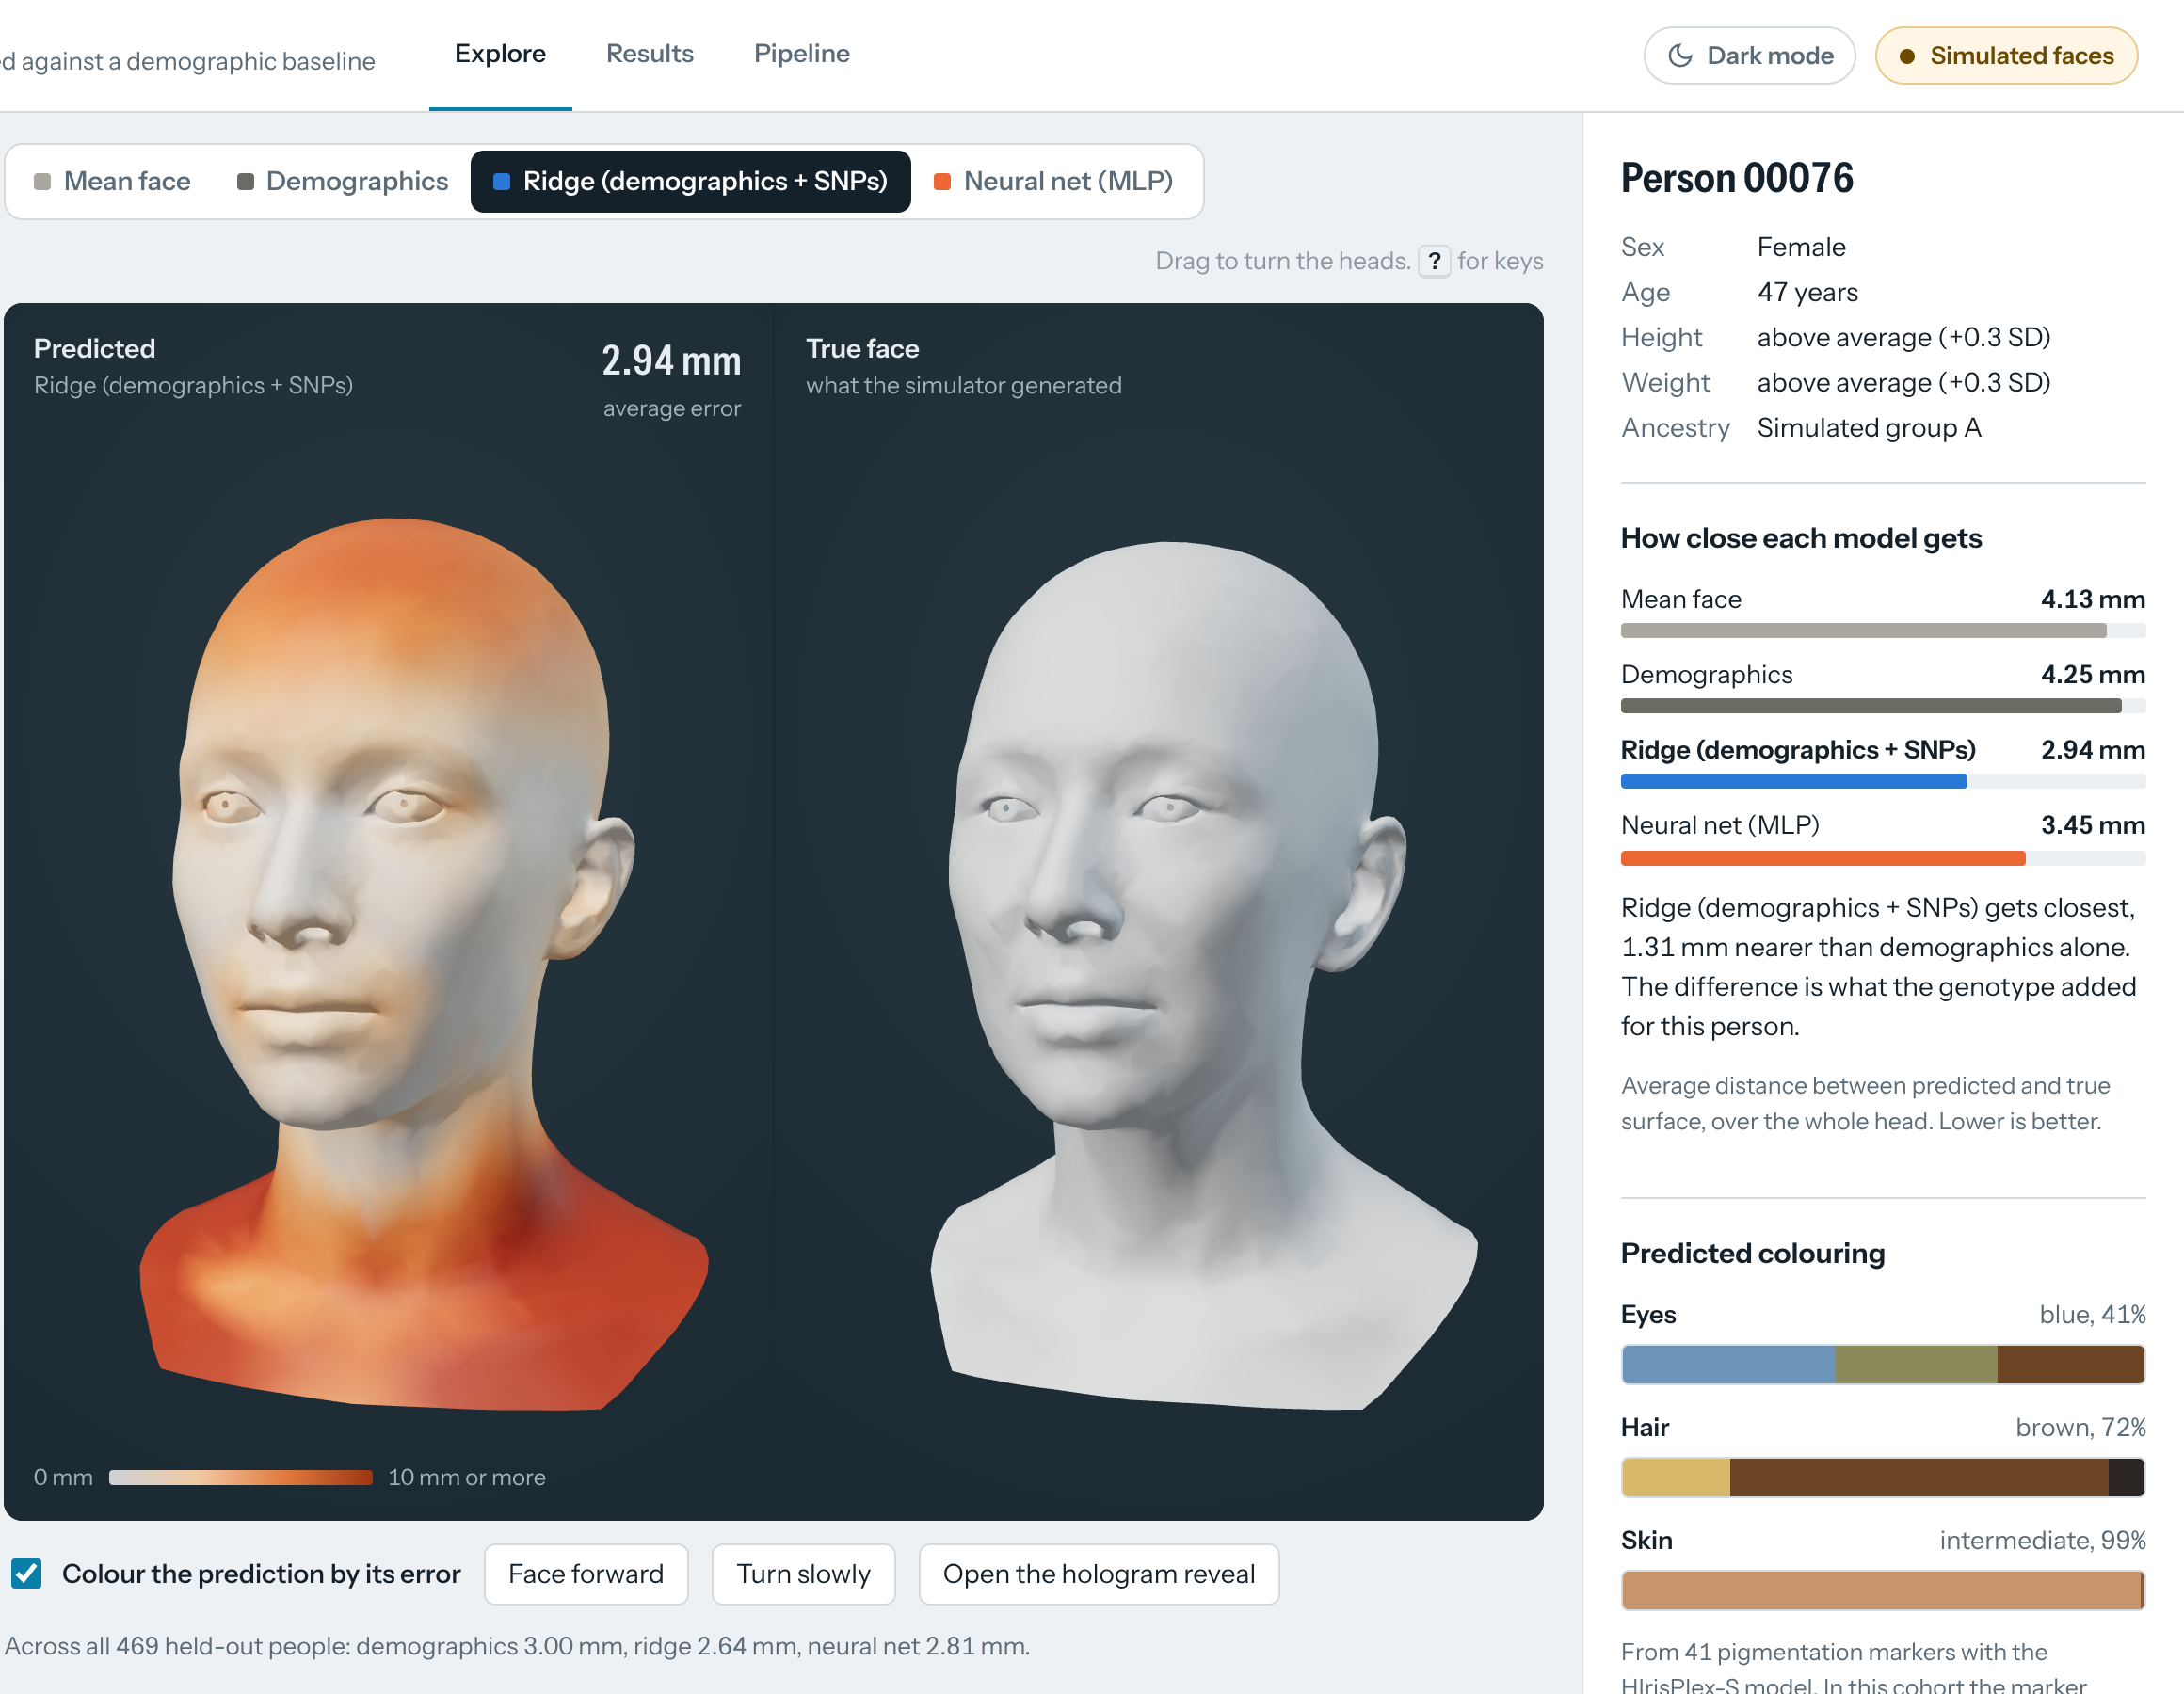
\includegraphics[width=\textwidth]{Figures/demo_explore_crop.png}
\caption{Explore view of the demonstrator, comparing the predicted and true faces for one held-out subject.}
\label{fig:demo-explore}
\end{figure}

\begin{figure}[!ht]
\centering
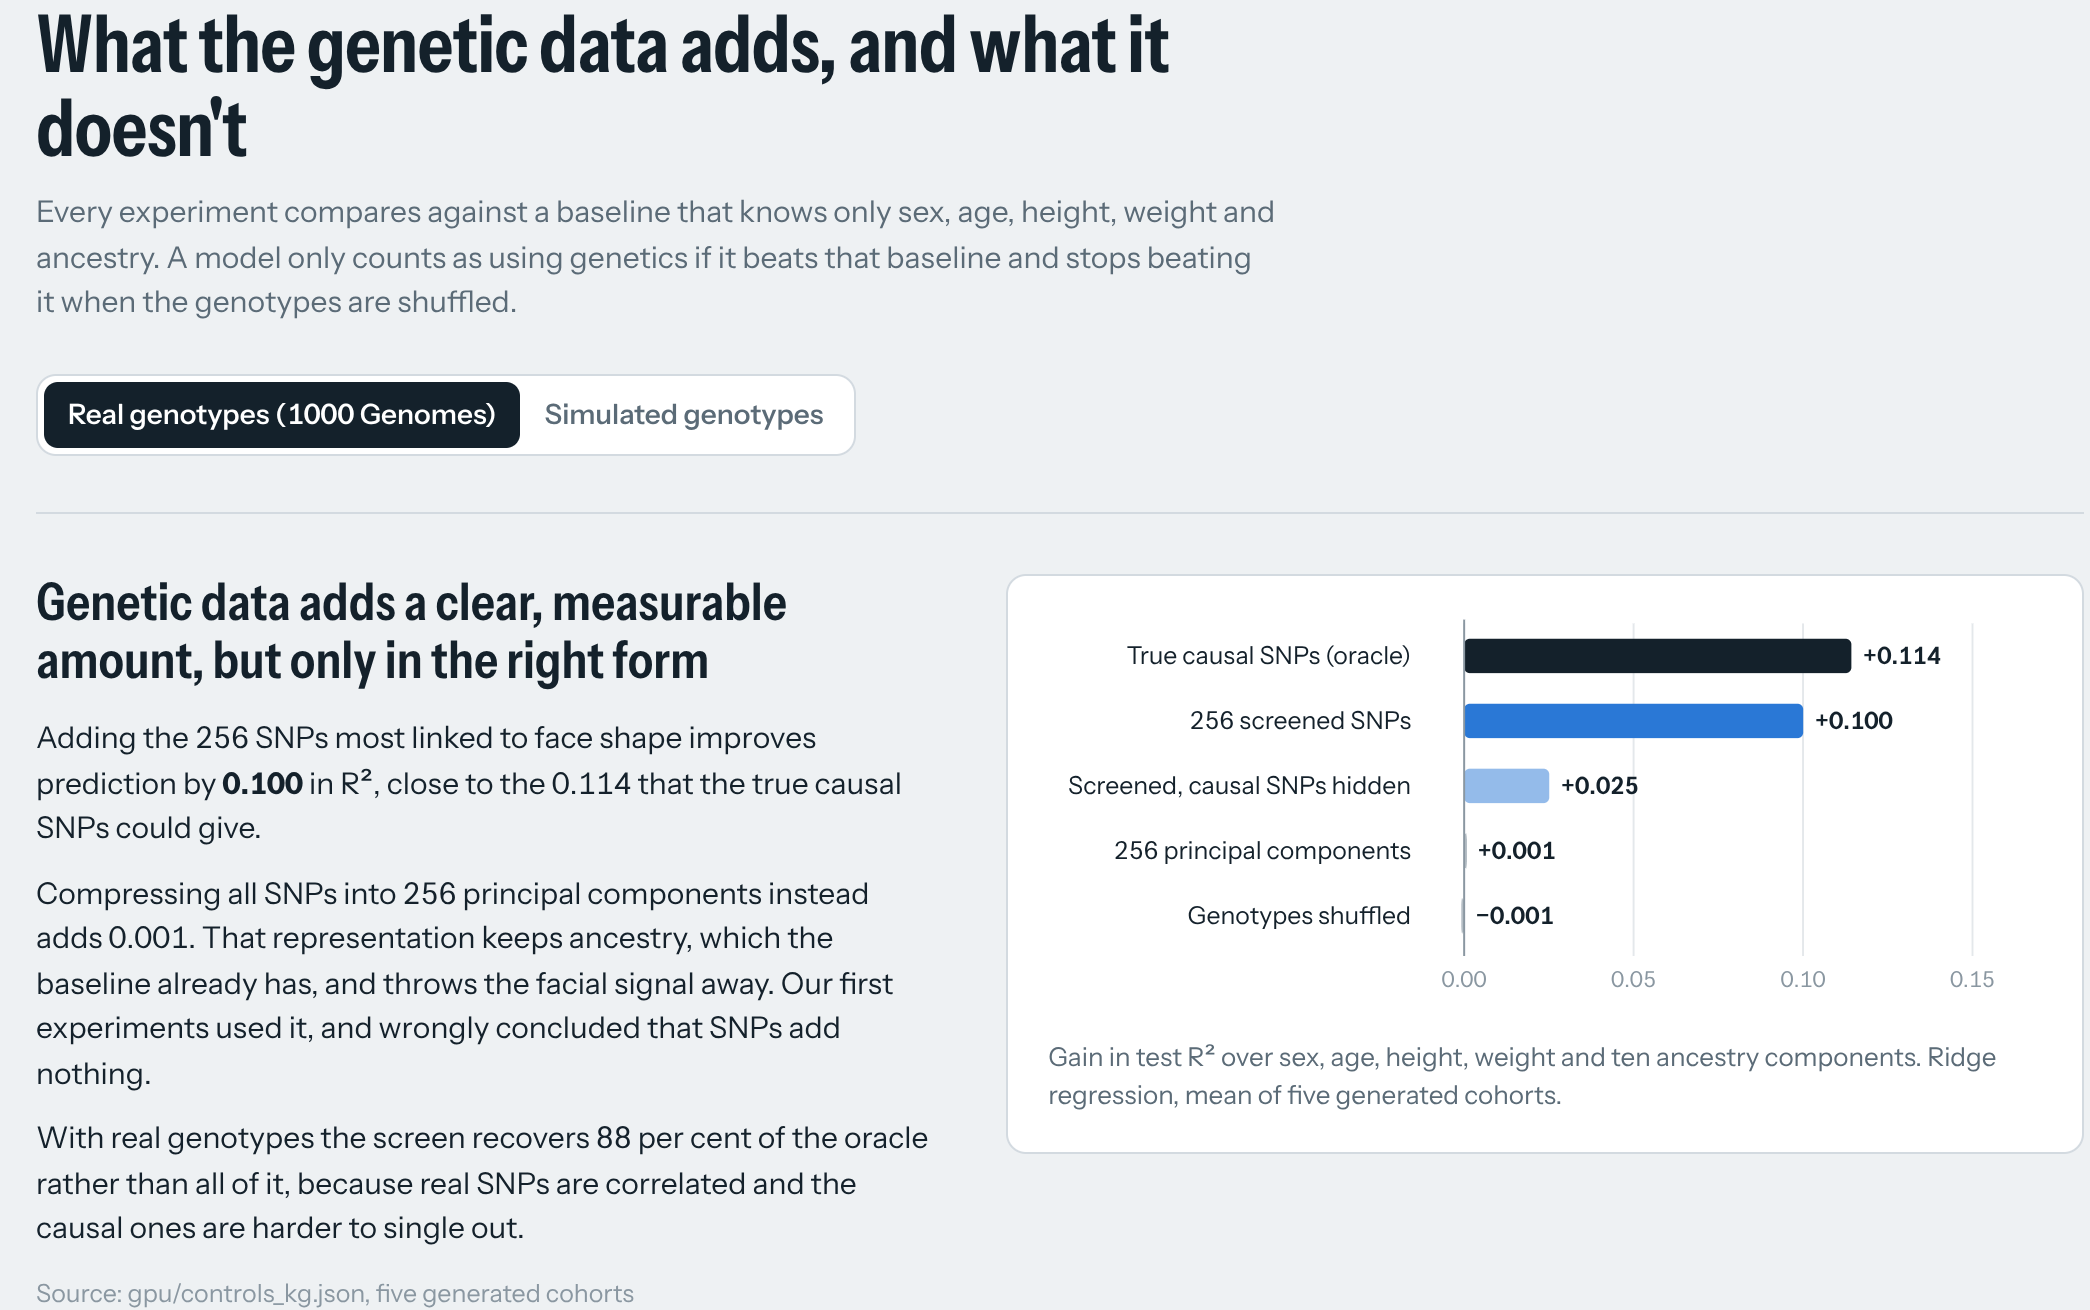
\includegraphics[width=\textwidth]{Figures/demo_results_crop.png}
\caption{Results view of the demonstrator, showing the first finding of the real-genotype experiment.}
\label{fig:demo-results}
\end{figure}

The page reads one precomputed data file and needs no server, so it also works when opened directly from disk. The file is written by an export script from the corrected pipeline of this chapter, using screened SNPs, the two-stage linear reference, and the face decoder with the same scale as the evaluation. Its figures therefore agree with Chapter~\ref{ch:results}, with the demographic baseline at $0.317$ in $R^2$ and $3.00$ millimetres of mesh error on the 469 test subjects. Two departures from the design of Chapter~\ref{ch:srs} should be noted. The face is the stand-in model rather than FLAME, for the reason given in Section~\ref{sec:impl-cohort}, and the baseline is compared through the list of errors and the model switch rather than as a third face on screen.

\section{Test Case Design and Description}
The test cases share the following attributes. Every test runs on simulated data only, so no controlled data is needed to execute the suite. Every test is automated, uses fixed random seeds, and is executed with a single command from the project root. The environment is Python~3 with the packages listed in the project requirements file, and no graphics card is required. The tests fall into three groups: unit tests of individual modules, integration tests that run a stage of the pipeline end to end, and scientific control tests that check a property the results depend on, such as the absence of leakage. Tables~\ref{tab:tc1} to~\ref{tab:tc6} describe six representative test cases in the recommended scheme, and Table~\ref{tab:tcall} lists the complete suite. The last four tests cover the real genotype panel of Section~\ref{sec:impl-1kg}. They run on a small fixture built by the test itself, with the allele cases that caused trouble in practice, so they need no download and no controlled data.


\begin{table}[H]
\caption{Test case TC-01: subject-level splits are disjoint.}
\label{tab:tc1}
\centering\small\setstretch{1.15}
\begin{tabular}{|llll|}
\hline
\multicolumn{4}{|c|}{\textbf{Dataset Builder}} \\ \hline
\multicolumn{4}{|c|}{\textbf{FR-05, NFR-01}} \\ \hline
\multicolumn{1}{|l|}{\textbf{Test Case ID:}} & \multicolumn{1}{l|}{TC-01} & \multicolumn{1}{l|}{\textbf{QA Test Engineer:}} & FaceCon project team \\ \hline
\multicolumn{1}{|l|}{\textbf{Test case Version:}} & \multicolumn{1}{l|}{1.0} & \multicolumn{1}{l|}{\textbf{Reviewed By:}} & FaceCon project team \\ \hline
\multicolumn{1}{|l|}{\textbf{Test Date:}} & \multicolumn{1}{l|}{13 November 2026} & \multicolumn{1}{l|}{\textbf{\begin{tabular}[c]{@{}l@{}}Use Case \\ Reference(s):\end{tabular}}} & UC-01, UC-03 \\ \hline
\multicolumn{1}{|l|}{\textbf{Revision History:}} & \multicolumn{3}{l|}{None} \\ \hline
\multicolumn{1}{|l|}{\textbf{Objective:}} & \multicolumn{3}{p{11.9cm}|}{Verify that no subject appears in more than one of the training, validation, and test sets, and that every subject is assigned.} \\ \hline
\multicolumn{1}{|l|}{\textbf{\begin{tabular}[c]{@{}l@{}}Product/Ver/\\ Module:\end{tabular}}} & \multicolumn{3}{p{11.9cm}|}{FaceCon prototype, simulated cohort generator, split construction.} \\ \hline
\multicolumn{1}{|l|}{\textbf{Environment:}} & \multicolumn{3}{p{11.9cm}|}{Python 3 with the project requirements, processor only, executed with pytest from the project root.} \\ \hline
\multicolumn{1}{|l|}{\textbf{Assumptions:}} & \multicolumn{3}{p{11.9cm}|}{The generator configuration is valid and the random seed is fixed.} \\ \hline
\multicolumn{1}{|l|}{\textbf{Pre-Requisite:}} & \multicolumn{3}{p{11.9cm}|}{None.} \\ \hline
\multicolumn{1}{|l|}{\textbf{Step No.}} & \multicolumn{1}{l|}{\textbf{Execution description}} & \multicolumn{2}{l|}{\textbf{Procedure result}} \\ \hline
\multicolumn{1}{|l|}{1} & \multicolumn{1}{p{5.6cm}|}{Generate a small simulated cohort of 500 subjects.} & \multicolumn{2}{p{6.3cm}|}{Cohort generated with three index sets.} \\ \hline
\multicolumn{1}{|l|}{2} & \multicolumn{1}{p{5.6cm}|}{Concatenate the three index sets and count unique subjects.} & \multicolumn{2}{p{6.3cm}|}{The number of unique subjects equals the cohort size.} \\ \hline
\multicolumn{1}{|l|}{3} & \multicolumn{1}{p{5.6cm}|}{Compare the total number of assigned indices with the cohort size.} & \multicolumn{2}{p{6.3cm}|}{The two numbers are equal, so there is no overlap and no omission.} \\ \hline
\multicolumn{4}{|p{15.2cm}|}{\textbf{Comments:} The controls script repeats this check on every full-size cohort as acceptance check A4.} \\ \hline
\multicolumn{4}{|c|}{\textbf{Passed}} \\ \hline
\end{tabular}
\end{table}

\begin{table}[H]
\caption{Test case TC-02: mesh error is computed at the generator's scale.}
\label{tab:tc2}
\centering\small\setstretch{1.15}
\begin{tabular}{|llll|}
\hline
\multicolumn{4}{|c|}{\textbf{Evaluator}} \\ \hline
\multicolumn{4}{|c|}{\textbf{FR-07, FR-08}} \\ \hline
\multicolumn{1}{|l|}{\textbf{Test Case ID:}} & \multicolumn{1}{l|}{TC-02} & \multicolumn{1}{l|}{\textbf{QA Test Engineer:}} & FaceCon project team \\ \hline
\multicolumn{1}{|l|}{\textbf{Test case Version:}} & \multicolumn{1}{l|}{1.0} & \multicolumn{1}{l|}{\textbf{Reviewed By:}} & FaceCon project team \\ \hline
\multicolumn{1}{|l|}{\textbf{Test Date:}} & \multicolumn{1}{l|}{13 November 2026} & \multicolumn{1}{l|}{\textbf{\begin{tabular}[c]{@{}l@{}}Use Case \\ Reference(s):\end{tabular}}} & UC-03, UC-06 \\ \hline
\multicolumn{1}{|l|}{\textbf{Revision History:}} & \multicolumn{3}{l|}{None} \\ \hline
\multicolumn{1}{|l|}{\textbf{Objective:}} & \multicolumn{3}{p{11.9cm}|}{Verify that the training harness decodes shape vectors with the same face basis and scale as the generator, so that mesh error in millimetres is correct.} \\ \hline
\multicolumn{1}{|l|}{\textbf{\begin{tabular}[c]{@{}l@{}}Product/Ver/\\ Module:\end{tabular}}} & \multicolumn{3}{p{11.9cm}|}{FaceCon prototype, training harness data loader and face model.} \\ \hline
\multicolumn{1}{|l|}{\textbf{Environment:}} & \multicolumn{3}{p{11.9cm}|}{Python 3 with the project requirements, processor only, executed with pytest from the project root.} \\ \hline
\multicolumn{1}{|l|}{\textbf{Assumptions:}} & \multicolumn{3}{p{11.9cm}|}{The stand-in face model file and the generated cohort are present.} \\ \hline
\multicolumn{1}{|l|}{\textbf{Pre-Requisite:}} & \multicolumn{3}{p{11.9cm}|}{Matched simulated cohort generated.} \\ \hline
\multicolumn{1}{|l|}{\textbf{Step No.}} & \multicolumn{1}{l|}{\textbf{Execution description}} & \multicolumn{2}{l|}{\textbf{Procedure result}} \\ \hline
\multicolumn{1}{|l|}{1} & \multicolumn{1}{p{5.6cm}|}{Load the cohort through the training harness.} & \multicolumn{2}{p{6.3cm}|}{The harness holds a face basis.} \\ \hline
\multicolumn{1}{|l|}{2} & \multicolumn{1}{p{5.6cm}|}{Load the face model through the generator's own loader.} & \multicolumn{2}{p{6.3cm}|}{The generator holds a face basis.} \\ \hline
\multicolumn{1}{|l|}{3} & \multicolumn{1}{p{5.6cm}|}{Compare the two bases element by element.} & \multicolumn{2}{p{6.3cm}|}{The bases agree within a relative tolerance of $10^{-4}$.} \\ \hline
\multicolumn{4}{|p{15.2cm}|}{\textbf{Comments:} Written after a review found that the harness omitted the identity scale and under-reported mesh error by a factor of 9.5. The defect is fixed.} \\ \hline
\multicolumn{4}{|c|}{\textbf{Passed}} \\ \hline
\end{tabular}
\end{table}

\begin{table}[H]
\caption{Test case TC-03: published lead SNPs are generated consistently.}
\label{tab:tc3}
\centering\small\setstretch{1.15}
\begin{tabular}{|llll|}
\hline
\multicolumn{4}{|c|}{\textbf{Simulated Cohort Generator}} \\ \hline
\multicolumn{4}{|c|}{\textbf{FR-01}} \\ \hline
\multicolumn{1}{|l|}{\textbf{Test Case ID:}} & \multicolumn{1}{l|}{TC-03} & \multicolumn{1}{l|}{\textbf{QA Test Engineer:}} & FaceCon project team \\ \hline
\multicolumn{1}{|l|}{\textbf{Test case Version:}} & \multicolumn{1}{l|}{1.0} & \multicolumn{1}{l|}{\textbf{Reviewed By:}} & FaceCon project team \\ \hline
\multicolumn{1}{|l|}{\textbf{Test Date:}} & \multicolumn{1}{l|}{13 November 2026} & \multicolumn{1}{l|}{\textbf{\begin{tabular}[c]{@{}l@{}}Use Case \\ Reference(s):\end{tabular}}} & UC-01 \\ \hline
\multicolumn{1}{|l|}{\textbf{Revision History:}} & \multicolumn{3}{l|}{None} \\ \hline
\multicolumn{1}{|l|}{\textbf{Objective:}} & \multicolumn{3}{p{11.9cm}|}{Verify that each published lead SNP is generated once even when it is the lead for several traits, and that the X-chromosome SNP respects sex.} \\ \hline
\multicolumn{1}{|l|}{\textbf{\begin{tabular}[c]{@{}l@{}}Product/Ver/\\ Module:\end{tabular}}} & \multicolumn{3}{p{11.9cm}|}{FaceCon prototype, injection of published association signals.} \\ \hline
\multicolumn{1}{|l|}{\textbf{Environment:}} & \multicolumn{3}{p{11.9cm}|}{Python 3 with the project requirements, processor only, executed with pytest from the project root.} \\ \hline
\multicolumn{1}{|l|}{\textbf{Assumptions:}} & \multicolumn{3}{p{11.9cm}|}{The effect table lists one lead SNP per trait.} \\ \hline
\multicolumn{1}{|l|}{\textbf{Pre-Requisite:}} & \multicolumn{3}{p{11.9cm}|}{Matched simulated cohort generated.} \\ \hline
\multicolumn{1}{|l|}{\textbf{Step No.}} & \multicolumn{1}{l|}{\textbf{Execution description}} & \multicolumn{2}{l|}{\textbf{Procedure result}} \\ \hline
\multicolumn{1}{|l|}{1} & \multicolumn{1}{p{5.6cm}|}{Read the marker identifiers and the marker matrix.} & \multicolumn{2}{p{6.3cm}|}{The number of columns equals the number of unique identifiers.} \\ \hline
\multicolumn{1}{|l|}{2} & \multicolumn{1}{p{5.6cm}|}{Select male subjects at the X-chromosome SNP.} & \multicolumn{2}{p{6.3cm}|}{No male subject has a dosage of one.} \\ \hline
\multicolumn{1}{|l|}{3} & \multicolumn{1}{p{5.6cm}|}{Select female subjects at the same SNP.} & \multicolumn{2}{p{6.3cm}|}{Dosages of one are present, as expected for two copies.} \\ \hline
\multicolumn{4}{|p{15.2cm}|}{\textbf{Comments:} Written after a review found a lead SNP generated as two unrelated columns and an X-chromosome SNP generated without regard to sex. Both defects are fixed.} \\ \hline
\multicolumn{4}{|c|}{\textbf{Passed}} \\ \hline
\end{tabular}
\end{table}

\begin{table}[H]
\caption{Test case TC-04: injected associations are recovered and no others.}
\label{tab:tc4}
\centering\small\setstretch{1.15}
\begin{tabular}{|llll|}
\hline
\multicolumn{4}{|c|}{\textbf{Simulated Cohort Generator}} \\ \hline
\multicolumn{4}{|c|}{\textbf{NFR-06}} \\ \hline
\multicolumn{1}{|l|}{\textbf{Test Case ID:}} & \multicolumn{1}{l|}{TC-04} & \multicolumn{1}{l|}{\textbf{QA Test Engineer:}} & FaceCon project team \\ \hline
\multicolumn{1}{|l|}{\textbf{Test case Version:}} & \multicolumn{1}{l|}{1.0} & \multicolumn{1}{l|}{\textbf{Reviewed By:}} & FaceCon project team \\ \hline
\multicolumn{1}{|l|}{\textbf{Test Date:}} & \multicolumn{1}{l|}{13 November 2026} & \multicolumn{1}{l|}{\textbf{\begin{tabular}[c]{@{}l@{}}Use Case \\ Reference(s):\end{tabular}}} & UC-03 \\ \hline
\multicolumn{1}{|l|}{\textbf{Revision History:}} & \multicolumn{3}{l|}{None} \\ \hline
\multicolumn{1}{|l|}{\textbf{Objective:}} & \multicolumn{3}{p{11.9cm}|}{Verify that an association scan adjusted for covariates detects the injected SNP and measurement pairs, and does not report pairs that were not injected.} \\ \hline
\multicolumn{1}{|l|}{\textbf{\begin{tabular}[c]{@{}l@{}}Product/Ver/\\ Module:\end{tabular}}} & \multicolumn{3}{p{11.9cm}|}{FaceCon prototype, association recovery check stored with the cohort.} \\ \hline
\multicolumn{1}{|l|}{\textbf{Environment:}} & \multicolumn{3}{p{11.9cm}|}{Python 3 with the project requirements, processor only, executed with pytest from the project root.} \\ \hline
\multicolumn{1}{|l|}{\textbf{Assumptions:}} & \multicolumn{3}{p{11.9cm}|}{Both the measurements and the dosages are adjusted for sex, age, age squared, height, weight, and ancestry before testing.} \\ \hline
\multicolumn{1}{|l|}{\textbf{Pre-Requisite:}} & \multicolumn{3}{p{11.9cm}|}{Matched simulated cohort generated.} \\ \hline
\multicolumn{1}{|l|}{\textbf{Step No.}} & \multicolumn{1}{l|}{\textbf{Execution description}} & \multicolumn{2}{l|}{\textbf{Procedure result}} \\ \hline
\multicolumn{1}{|l|}{1} & \multicolumn{1}{p{5.6cm}|}{Test all 260 pairs of SNP and measurement.} & \multicolumn{2}{p{6.3cm}|}{A p-value is obtained for every pair.} \\ \hline
\multicolumn{1}{|l|}{2} & \multicolumn{1}{p{5.6cm}|}{Apply a Bonferroni threshold to the 14 injected pairs (positive control).} & \multicolumn{2}{p{6.3cm}|}{All 14 are detected with the published direction of effect.} \\ \hline
\multicolumn{1}{|l|}{3} & \multicolumn{1}{p{5.6cm}|}{Apply the same threshold to the 246 pairs that were not injected (negative control).} & \multicolumn{2}{p{6.3cm}|}{None is detected, and 2.8 per cent fall below 0.05, which is consistent with chance.} \\ \hline
\multicolumn{4}{|p{15.2cm}|}{\textbf{Comments:} The acceptance rule requires at least 80 per cent of injected pairs to be detected and no false detection.} \\ \hline
\multicolumn{4}{|c|}{\textbf{Passed}} \\ \hline
\end{tabular}
\end{table}

\begin{table}[H]
\caption{Test case TC-05: SNP signal is found when planted and absent when broken.}
\label{tab:tc5}
\centering\small\setstretch{1.15}
\begin{tabular}{|llll|}
\hline
\multicolumn{4}{|c|}{\textbf{Controls and Baseline Ladder}} \\ \hline
\multicolumn{4}{|c|}{\textbf{FR-09, NFR-06}} \\ \hline
\multicolumn{1}{|l|}{\textbf{Test Case ID:}} & \multicolumn{1}{l|}{TC-05} & \multicolumn{1}{l|}{\textbf{QA Test Engineer:}} & FaceCon project team \\ \hline
\multicolumn{1}{|l|}{\textbf{Test case Version:}} & \multicolumn{1}{l|}{1.0} & \multicolumn{1}{l|}{\textbf{Reviewed By:}} & FaceCon project team \\ \hline
\multicolumn{1}{|l|}{\textbf{Test Date:}} & \multicolumn{1}{l|}{13 November 2026} & \multicolumn{1}{l|}{\textbf{\begin{tabular}[c]{@{}l@{}}Use Case \\ Reference(s):\end{tabular}}} & UC-03 \\ \hline
\multicolumn{1}{|l|}{\textbf{Revision History:}} & \multicolumn{3}{l|}{None} \\ \hline
\multicolumn{1}{|l|}{\textbf{Objective:}} & \multicolumn{3}{p{11.9cm}|}{Verify that screened SNPs improve prediction beyond covariates and ancestry components when a genetic share is planted, and that the improvement disappears when the genotype rows are shuffled.} \\ \hline
\multicolumn{1}{|l|}{\textbf{\begin{tabular}[c]{@{}l@{}}Product/Ver/\\ Module:\end{tabular}}} & \multicolumn{3}{p{11.9cm}|}{FaceCon prototype, controls script.} \\ \hline
\multicolumn{1}{|l|}{\textbf{Environment:}} & \multicolumn{3}{p{11.9cm}|}{Python 3 with the project requirements, processor only, executed with pytest from the project root.} \\ \hline
\multicolumn{1}{|l|}{\textbf{Assumptions:}} & \multicolumn{3}{p{11.9cm}|}{A genetic share of 0.20 is planted. Screening and all scaling use the training set only.} \\ \hline
\multicolumn{1}{|l|}{\textbf{Pre-Requisite:}} & \multicolumn{3}{p{11.9cm}|}{None. The test generates its own cohort of 1{,}000 subjects.} \\ \hline
\multicolumn{1}{|l|}{\textbf{Step No.}} & \multicolumn{1}{l|}{\textbf{Execution description}} & \multicolumn{2}{l|}{\textbf{Procedure result}} \\ \hline
\multicolumn{1}{|l|}{1} & \multicolumn{1}{p{5.6cm}|}{Fit the ladder on the generated cohort (positive control).} & \multicolumn{2}{p{6.3cm}|}{The gain from screened SNPs exceeds 0.03 in $R^2$.} \\ \hline
\multicolumn{1}{|l|}{2} & \multicolumn{1}{p{5.6cm}|}{Shuffle the genotype rows and fit again (negative control).} & \multicolumn{2}{p{6.3cm}|}{The gain is below 0.01 in $R^2$.} \\ \hline
\multicolumn{4}{|p{15.2cm}|}{\textbf{Comments:} The full-size version of this test, with five cohorts and confidence intervals, is reported in Chapter~\ref{ch:results}.} \\ \hline
\multicolumn{4}{|c|}{\textbf{Passed}} \\ \hline
\end{tabular}
\end{table}

\begin{table}[H]
\caption{Test case TC-06: appearance predictions are not degenerate.}
\label{tab:tc6}
\centering\small\setstretch{1.15}
\begin{tabular}{|llll|}
\hline
\multicolumn{4}{|c|}{\textbf{Appearance Module}} \\ \hline
\multicolumn{4}{|c|}{\textbf{FR-11, FR-12}} \\ \hline
\multicolumn{1}{|l|}{\textbf{Test Case ID:}} & \multicolumn{1}{l|}{TC-06} & \multicolumn{1}{l|}{\textbf{QA Test Engineer:}} & FaceCon project team \\ \hline
\multicolumn{1}{|l|}{\textbf{Test case Version:}} & \multicolumn{1}{l|}{1.0} & \multicolumn{1}{l|}{\textbf{Reviewed By:}} & FaceCon project team \\ \hline
\multicolumn{1}{|l|}{\textbf{Test Date:}} & \multicolumn{1}{l|}{13 November 2026} & \multicolumn{1}{l|}{\textbf{\begin{tabular}[c]{@{}l@{}}Use Case \\ Reference(s):\end{tabular}}} & UC-03, UC-05 \\ \hline
\multicolumn{1}{|l|}{\textbf{Revision History:}} & \multicolumn{3}{l|}{None} \\ \hline
\multicolumn{1}{|l|}{\textbf{Objective:}} & \multicolumn{3}{p{11.9cm}|}{Verify that the appearance module does not assign nearly every subject to one category for eye, hair, or skin colour.} \\ \hline
\multicolumn{1}{|l|}{\textbf{\begin{tabular}[c]{@{}l@{}}Product/Ver/\\ Module:\end{tabular}}} & \multicolumn{3}{p{11.9cm}|}{FaceCon prototype, appearance module and marker generation.} \\ \hline
\multicolumn{1}{|l|}{\textbf{Environment:}} & \multicolumn{3}{p{11.9cm}|}{Python 3 with the project requirements, processor only, executed with pytest from the project root.} \\ \hline
\multicolumn{1}{|l|}{\textbf{Assumptions:}} & \multicolumn{3}{p{11.9cm}|}{The marker allele frequencies stored with the project are used.} \\ \hline
\multicolumn{1}{|l|}{\textbf{Pre-Requisite:}} & \multicolumn{3}{p{11.9cm}|}{Matched simulated cohort generated.} \\ \hline
\multicolumn{1}{|l|}{\textbf{Step No.}} & \multicolumn{1}{l|}{\textbf{Execution description}} & \multicolumn{2}{l|}{\textbf{Procedure result}} \\ \hline
\multicolumn{1}{|l|}{1} & \multicolumn{1}{p{5.6cm}|}{Predict eye, hair, and skin colour for every subject.} & \multicolumn{2}{p{6.3cm}|}{A category is returned for each trait and subject.} \\ \hline
\multicolumn{1}{|l|}{2} & \multicolumn{1}{p{5.6cm}|}{Compute the share of the most frequent category for each trait.} & \multicolumn{2}{p{6.3cm}|}{The share is below 90 per cent for all three traits.} \\ \hline
\multicolumn{4}{|p{15.2cm}|}{\textbf{Comments:} Written after regenerating the cohort silently reset the marker frequencies and every subject was predicted to have red hair. This test checks plausibility of the simulated inputs and is not a measure of accuracy.} \\ \hline
\multicolumn{4}{|c|}{\textbf{Passed}} \\ \hline
\end{tabular}
\end{table}

\begin{table}[H]
\centering
\caption{The complete automated test suite. All 44 test cases passed in the final run.}
\label{tab:tcall}
\small\setstretch{1.1}
\begin{tabular}{|p{0.9cm}|p{9.3cm}|p{1.9cm}|p{1.9cm}|}
\hline
\textbf{No.} & \textbf{What the test verifies} & \textbf{Type} & \textbf{Detailed in} \\ \hline
T01 & Published lead SNPs generated once, with sex-aware X chromosome & Control & TC-03 \\ \hline
T02 & Injected associations recovered, with no false detections & Control & TC-04 \\ \hline
T03 & Feature matrices have the expected shapes & Unit & --- \\ \hline
T04 & Configuration loads and variance shares sum to one & Unit & --- \\ \hline
T05 & Named random streams are reproducible and independent & Unit & --- \\ \hline
T06 & Dosages take only the values 0, 1, and 2, and shapes are consistent & Unit & --- \\ \hline
T07 & Splits are disjoint and cover every subject & Control & TC-01 \\ \hline
T08 & Realised variance shares match the configuration & Integration & --- \\ \hline
T09 & Saving and reloading a cohort returns identical data & Integration & --- \\ \hline
T10 & Generation is bit-for-bit unchanged when no architecture block is set & Control & --- \\ \hline
T11 & The committed real-match cohort regenerates exactly from its seed & Control & --- \\ \hline
T12 & Quality-control statistics are fitted on the training set only & Control & --- \\ \hline
T13 & Baselines rank sensibly, with the mean face near zero & Integration & --- \\ \hline
T14 & Full evaluation returns every metric for every model & Integration & --- \\ \hline
T15 & Planted signal is recovered above a shuffled-label control & Control & --- \\ \hline
T16 & Mesh error uses the generator's face basis and scale & Control & TC-02 \\ \hline
T17 & Appearance predictions are not degenerate & Control & TC-06 \\ \hline
T18 & SNP signal found when planted and absent when shuffled & Control & TC-05 \\ \hline
T19 & Genotype files are written and read back identically, including missing calls & Unit & --- \\ \hline
T20 & Published alleles are matched to the panel by the documented rules, and ambiguous ones are refused & Unit & --- \\ \hline
T21 & Real genotypes run end to end, from panel to features to controls & Integration & --- \\ \hline
T22 & Sparse genetic effects touch only the chosen shape dimensions & Control & --- \\ \hline
T23--T25 & Dominance and interaction shares are realised at the configured sizes, once for each of the three architectures & Integration & --- \\ \hline
T26 & Heterozygote coding is correct when dosages have been mean-imputed & Unit & --- \\ \hline
T27 & Non-additive weights stay sparse, one row at a time & Unit & --- \\ \hline
T28 & The architecture block is validated, and impossible fractions are refused & Unit & --- \\ \hline
T29 & The processor-only harness refuses non-additive configurations rather than running them wrongly & Control & --- \\ \hline
T30--T32 & Correctly coded non-additive signal scores above a shuffled control, once for each of the three architectures & Control & --- \\ \hline
T33 & A zero genetic share reports nothing through the non-additive rows & Control & --- \\ \hline
T34 & The column-count cost of the non-additive oracle on an additive target is a cost, and keeps its measured size & Control & --- \\ \hline
T35 & The two-degree-of-freedom screen beats the additive screen on a dominance cohort & Control & --- \\ \hline
T36 & A stored split is reproduced exactly from its split seed & Control & --- \\ \hline
T37 & A different split seed redraws the split and still partitions the cohort & Control & --- \\ \hline
T38 & The generator refuses to overwrite the tracked cohort without an explicit override & Control & --- \\ \hline
T39 & The rotation parameterisation returns genuine rotations & Unit & --- \\ \hline
T40 & Scan fitting recovers the shape vector of a noise-free synthetic scan & Integration & --- \\ \hline
T41 & The iterative stage improves on the closed-form landmark warm start & Integration & --- \\ \hline
T42 & A mesh of noise gives a far larger fit residual than a real face & Control & --- \\ \hline
T43 & Scan fitting is reproducible from its seed & Unit & --- \\ \hline
T44 & The fitting layer works in millimetres, applying the model's scale & Unit & --- \\ \hline
\end{tabular}
\end{table}


\section{Test Metrics}
Table~\ref{tab:tmetrics} summarises the test metrics for the suite, and Table~\ref{tab:ttrace} traces the requirements of Chapter~\ref{ch:srs} to the tests that cover them.

\begin{table}[H]
\centering
\caption{Test metrics for the FaceCon prototype.}
\label{tab:tmetrics}
\small
\begin{tabular}{|P{5.2cm}|P{9.3cm}|}
\hline
\textbf{Metric} & \textbf{Value} \\ \hline
Number of test cases & 44 automated test cases \\ \hline
Number of test cases passed & 44 \\ \hline
Number of test cases failed & 0 in the final run \\ \hline
Test case defect density & 0 per cent in the final run, computed as failed test cases divided by executed test cases \\ \hline
Test case effectiveness & 4 of the 6 defects found during this phase are now guarded by a dedicated test (67 per cent). The defects themselves were found by a manual review, by the oracle control, and by a negative control, after which the tests were written \\ \hline
Acceptance checks & All acceptance checks of the controls script passed on the additive simulated and real-genotype cohorts and on the non-additive simulated cohorts, and the checks of the experiment runner passed in every run. On the real-genotype mixed cohort one positive control failed, as Section~\ref{sec:res-nonadd-real} reports, and its threshold was not lowered \\ \hline
\end{tabular}
\end{table}

The defects referred to in Table~\ref{tab:tmetrics} are reported openly because finding them is part of the result. They were a feature step that discarded the planted signal, a scale error that under-reported mesh error by a constant factor, a regeneration step that reset the appearance marker frequencies, a lead SNP that was generated twice as two unrelated columns, an X-chromosome SNP that ignored sex, and a linear reference that penalised the demographic covariates alongside the SNPs and so scored below the demographic baseline under permutation. The first two affected reported numbers and are discussed in Chapter~\ref{ch:results}. The sixth was found by its own negative control before any result depended on it, and is described in Section~\ref{sec:res-real}. Four have regression tests or acceptance checks of their own, and the first is covered by the oracle control and the second by test case TC-02.

\begin{table}[H]
\centering
\caption{Traceability from requirements to test cases.}
\label{tab:ttrace}
\small
\begin{tabular}{|P{2.2cm}|P{6.6cm}|P{5.7cm}|}
\hline
\textbf{Requirement} & \textbf{Subject of the requirement} & \textbf{Covering tests (Table~\ref{tab:tcall})} \\ \hline
FR-01 & Subject-by-SNP dosage matrix & T06, T09 \\ \hline
FR-05, NFR-01 & Subject-level splits with no overlap & T07, and acceptance check A4 \\ \hline
FR-06 & Training and running the models & T12, T13, T18 \\ \hline
FR-07 & Decoding a shape vector to a mesh & T16 \\ \hline
FR-08 & Evaluation metrics & T14, T16 \\ \hline
FR-09 & Comparison against baselines & T13, T18 \\ \hline
FR-11, FR-12 & Appearance prediction from marker SNPs & T10, T11, T17 \\ \hline
NFR-02 & Statistics fitted on training data only & T12 \\ \hline
NFR-03 & Configuration and seeds & T04, T05, T09 \\ \hline
NFR-06 & Honest reporting with controls & T15, T18, and acceptance checks A1 to A3 \\ \hline
FR-02 & Real genotype QC and allele alignment & T19, T20, T21, on the 1000 Genomes panel. QC of the 3DFN files is not yet testable \\ \hline
FR-03, FR-04 & Scan ingestion and FLAME registration & Not yet testable, since they require the real data \\ \hline
\end{tabular}
\end{table}

\section{Conclusion}
This chapter described the prototype that implements the FaceCon methodology: a simulated cohort generator matched to the public description of the target study, a real genotype panel, a stand-in face model, published association signals, the appearance module, two SNP representations, four baselines, four neural models, and a set of controls. It also described a second cohort in which the simulated genotypes are replaced by real ones from the 1000 Genomes Project, and the 44 automated test cases, all of which pass, traced to the requirements. Genotype QC and allele alignment are now exercised on real files, although not yet on the 3DFN genotypes themselves. FLAME registration of real scans is implemented and validated on synthetic scans, within $0.5$ mm of the shape vector they were generated from, but has not been run on real scans. The appearance module reproduces the public calculator, and a check against self-reported eye colour in an open cohort is implemented but not yet run. With the implementation verified, Chapter~\ref{ch:results} reports the experiments run on it.
